Given X and Y be two continuous random variables with the joint probability density function
\begin{align}
    f\left(x,y\right)=\begin{cases}
    2 \quad  0<x+y<1 ,x>0 ,y>0\\
    0 \quad  \textrm{elsewhere}\\
    \end{cases}
\end{align}
% \begin{figure}[h]
%     \centering
%     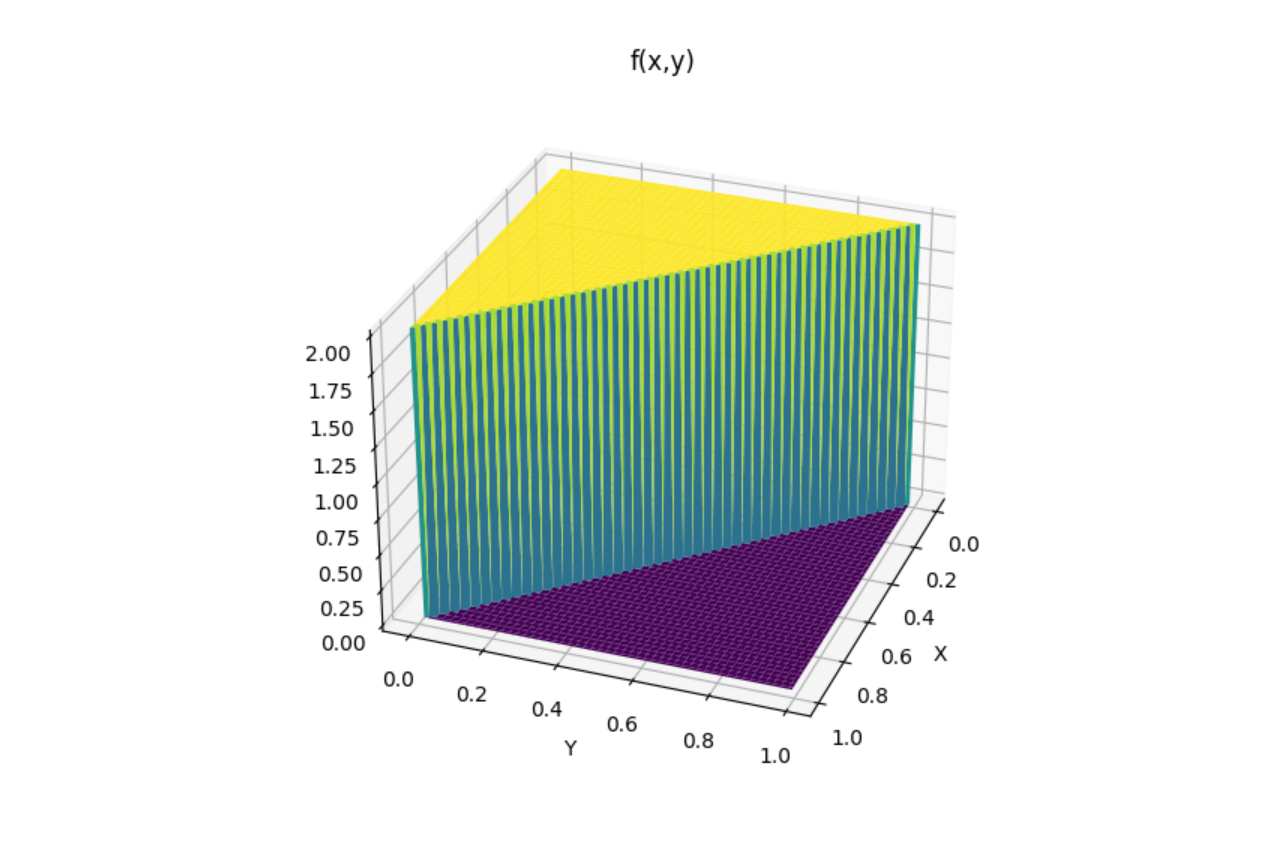
\includegraphics[scale=0.2]{f(x,y)_graph.png}
%     \caption{$f\left(x,y\right)$}
%     \label{ec/75/fig:f(x,y)}
% \end{figure}

we know that
\begin{align}
    P\left(\left(x,y\right)\in A\right)=\int \int _{A}f\left(x,y\right) dx dy \quad  A \in \mathbb{R}^2
\end{align}
from given information\\
for positive $x$ and $y$
\begin{align}
    0<x+y<\dfrac{1}{2}  \Rightarrow 0<x<\dfrac{1}{2}-y
\end{align}
so using eq(0.0.3)
\begin{align}
    P\left(x+y < \dfrac{1}{2}\right)=\int_{0}^{\frac{1}{2}} \int _{0}^{\frac{1}{2}-y}f(x,y) dx dy\\
    =\int_{0}^{\frac{1}{2}} \int _{0}^{\frac{1}{2}-y} 2 \quad dx dy
    =\int_{0}^{\frac{1}{2}} \left(  2 x \quad \big|_{0}^{\frac{1}{2}-y} \right)  dy\\
    =\int_{0}^{\frac{1}{2}}   2 \left(\frac{1}{2}-y\right) \quad    dy
    =2\left( \frac{1}{2} y - \frac{y^2}{2}  \right) \big|_{0}^{\frac{1}{2}}\\
    = \left( \frac{1}{2} - \frac{1}{4}\right) = \frac{1}{4} 
\end{align}
Therefore 
\begin{align}
    P\left(X+Y<\dfrac{1}{2}\right)=\dfrac{1}{4}
\end{align}
\begin{align}
\intertext{volume under the graph which contains the region} X+Y<\dfrac{1}{2} \quad \text{gives us} \quad P\left(X+Y<\dfrac{1}{2}\right) \\
 P\left(X+Y<\dfrac{1}{2}\right)= \text{Area of the base . height}
 \end{align}
 
Area of the base triangle is 
\begin{align}
 \dfrac{1}{2}.\textit{height}.\textit{base} =\dfrac{1}{2}.\dfrac{1}{2}.\dfrac{1}{2}
 \end{align}
 \begin{align}
\text{volume = Area . height}=\dfrac{1}{8}. 2= \dfrac{1}{4}
\end{align}
%The volume under the graph which contains the region $X+Y<\dfrac{1}{2}$ %gives us $P\left(x+y<\dfrac{1}{2}\right)$\\
%$P\left(x+y<\dfrac{1}{2}\right)=$ Area of the base . height\\
%Area of the base triangle is $\dfrac{1}{2}.\textit{height}.\textit{base}$%$= \dfrac{1}{2}.\dfrac{1}{2}.\dfrac{1}{2}$\\
%volume = Area . height $= \dfrac{1}{8}. 2= \dfrac{1}{4}$

\begin{figure}[h]
    \centering
    %\columnwidth
    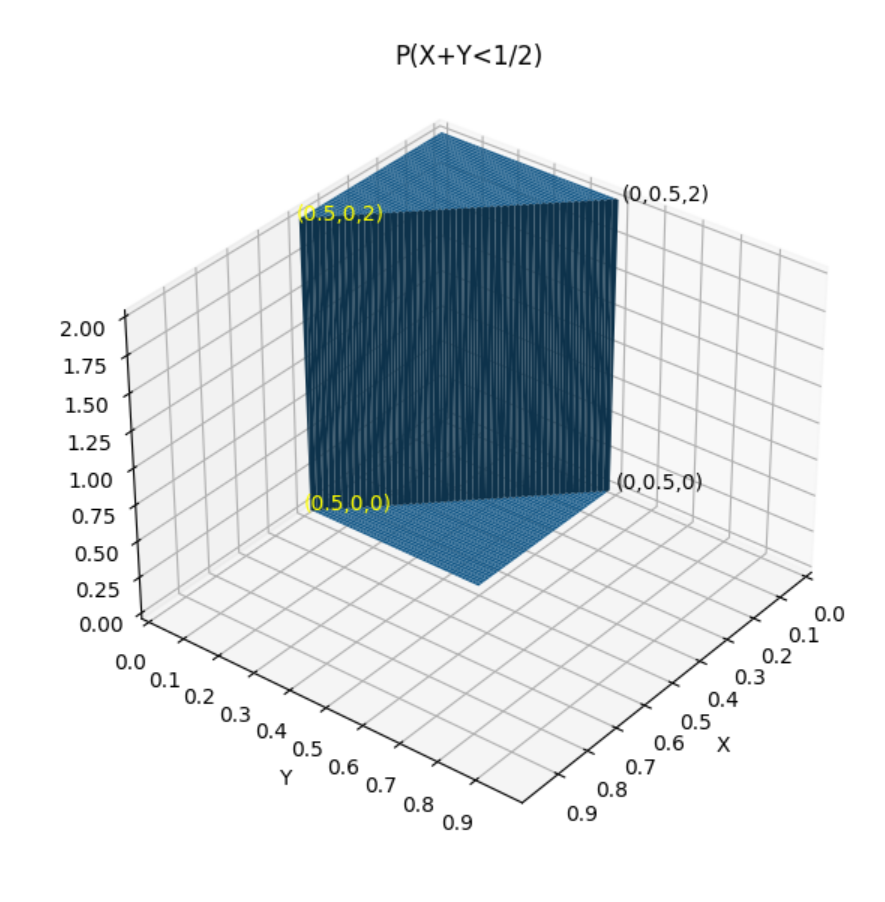
\includegraphics[width=\columnwidth]{solutions/ec/75/P(x+y_2)_graph.png}
    \caption{$P\left(x+y<\dfrac{1}{2}\right)$}
    \label{ec/75/fig:p(x+y<1/2)}
\end{figure}


